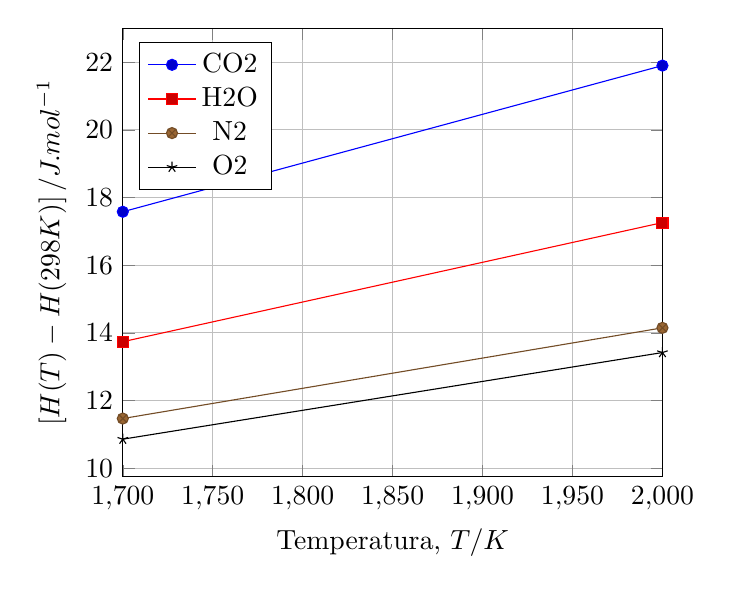
\begin{tikzpicture}
    \begin{axis}
        [
            grid = major,
            xlabel = {Temperatura, $T/\si{K}$},
            ylabel = {$\left[H(T) - H(\qty{298}{K})\right]/\si{J.mol^{-1}}$},
            xmajorgrids,
            legend pos = north west, 
            xmin=1700,xmax=2000
        ]
    \addplot coordinates
        {
            (1700,17.58)
            (2000,21.90)
        };
    \addplot coordinates
        {
            (1700,13.74)
            (2000,17.26)
        };
    \addplot coordinates
        {
            (1700,11.47)
            (2000,14.15)
        };
    \addplot coordinates
        {
            (1700,10.86)
            (2000,13.42)
        };
    \legend{{\ce{CO2}},{\ce{H2O}},{\ce{N2}}, {\ce{O2}}}
    \end{axis}
\end{tikzpicture}